% !TeX root = ../../thesis.tex

\section{Security}

\autoref{fig:windows-startup-process} gives an overview over the security within the Windows startup process.
With Secure Boot starting the process and Trusted Boot enventually taking over.
We do not cover Measured Boot in this thesis.

\begin{figure}[phtb]
    \centering
    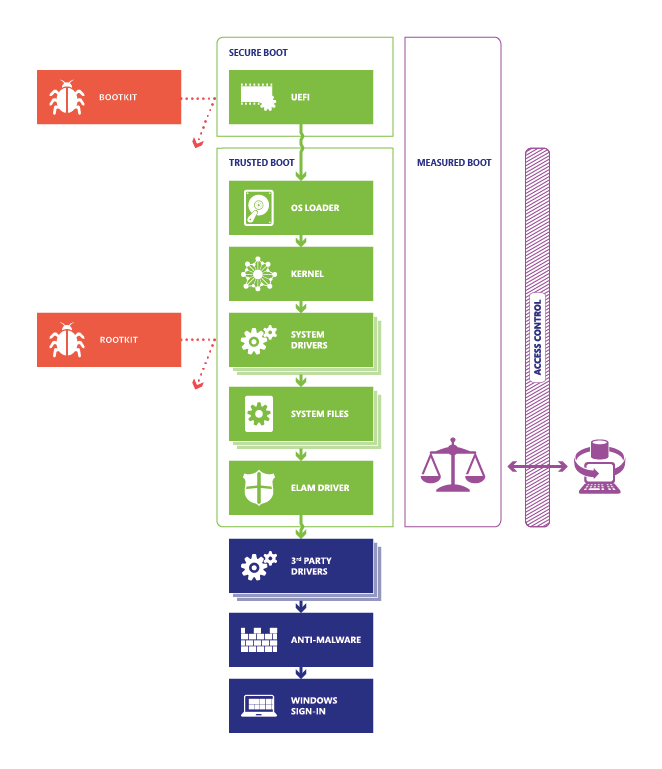
\includegraphics[width=1.0\textwidth]{windows/windows_startup_process.png}
    \caption{Windows startup process (taken from \cite{microsoft-secure-the-windows-boot-process})}
    \label{fig:windows-startup-process}
\end{figure}

\subsection{Secure Boot}

Devices shipping with Windows 11 must have Secure Boot enabled by default \cite{microsoft-windows-minimum-hardware-requirements-overview}.
Windows certified devices generally must allow users to enroll custom keys and signature \acp{DB} (to allow executioon of non\-/Windows bootloaders), aditionally a user should be able to completely disable secure boot.
Windows offers two signature \acp{DB} the \emph{Microsoft Windows Production PCA 2011} required for the Windows boot process and \emph{Microsoft Corporation \ac{UEFI} \ac{CA} 2011}, which is reserved for third party executables signed at Microsoft's discretion after manual review \cite{microsoft-uefi-signing}.
Microsoft advises to only allow other third party \ac{UEFI} applications if necessary and even mandates the exclusion of \acp{DB} other than \emph{Microsoft Windows Production PCA 2011} on Secured\-/core \acp{PC} \cite{microsoft-secure-the-windows-boot-process}.

\subsection{Trusted Boot}

Trusted Boot picks up where Secure Boot left off and maintains the code integrity chain through the kernel into the Windows startup process.
\ac{KMCI} verifies the digital signature of Windows boot components, including boot drivers, startup files and the \ac{ELAM} driver \cite{microsoft-trusted-boot}.
\ac{ELAM} provides antimalware software developers an interface to be intialized early in the boot process, before other third\-/party components, to monitor the subsequent boot process \cite{micosoft-windows-elam}.
\cite{understanding-windows-trusted-boot} gives a detailed walkthrough of the trusted boot process.

Microsoft can also leverage hardware virtualization features called \ac{VSM} for \ac{VBS}.
This allows for \ac{HVCI} where the \ac{CI} checks are taken out of the kernel environment and are now be performed from within the isolated hypervisor\-/based security environment \cite{micosoft-windows-oem-vbs}.

Formerly the term \emph{Device Guard} was used to promote the two security related features \ac{HVCI} and \ac{WDAC} (restricts execution of user level applcations).
Microsoft has since retired the term to prevent confusion, as there is no direct dependency between the two \cite{microsoft-windows-no-longer-device-guard}.

\subsection{\acf{BDE}}
\label{sec:windows:security:bde}

Windows is only able to enforce security policies when it is active, leaving the system vulnerable when accessed from outside of the \ac{OS} \cite[Section 9]{windows-internals-6-part2}.
Windows uses BitLocker, an integrated \ac{FVE}, aimed to protect system files and data from unauthorized accecss while at rest \cite{microsoft-bitlocker-overview}.
It also serves as a mechanism to verify boot integrity when used with in combination of a \ac{TPM} \cite[Section 9]{windows-internals-6-part2}.
The en- and decryption of the volume is done by a filter driver beneath the \ac{NTFS} driver as shown in \autoref{fig:bitlocker-volume-access-driver-stack}.
The \ac{NTFS} driver translates file and directory access into block-wise operations on the volume.
The filter driver then receives these block operations, encrypting blocks on write and decrypting blocks on read, while they pass through it.
This results in en- and decryption, that is entirely transparent to the \ac{NTFS} driver, making the underlying volume appear decrypted \cite[Section 9]{windows-internals-6-part2}.
The encryption of each block is done using a modified version of the \ac{AES}128 and \ac{AES}256 cypher \cite[Section 9]{windows-internals-6-part2}.
A \ac{FVEK} is used in combination with the block index as input for the algorithm, resulting in an entirely different output for two blocks with identical data \cite[Section 9]{windows-internals-6-part2}.
The \ac{FVEK} is encrypted with a \ac{VMK} which is in turn encrypted with multiple protectors.
These encrypted versions of the \ac{VMK} are stored together with the encrypted \ac{FVEK} in an unencrypted meta data portion at the beginning of the BitLocker protected volume \cite[Section 9]{windows-internals-6-part2}.
The \ac{VMK} can be encrypted by the following protectors:

\begin{figure}[htb]%
    \centering
    \includesvg[width=0.5\textwidth]{bitlocker_volume_access_driver_stack.drawio.svg}
    \caption{BitLocker Volume Access Driver Stack (inspired by \cite[Figure 9-24]{windows-internals-6-part2})}%
    \label{fig:bitlocker-volume-access-driver-stack}%
\end{figure}

\begin{description}
    \item[Startup key] The Startup key can be storead on removable media such as a \ac{USB} stick and serves as physical proof of ownership.
        The removable media contains a \program{.bek} file, that is named with a \ac{GUID} corresponding to BitLocker meta data entry, as it it possible to have multiple start up keys for the same volume \cite[Section 2.6]{bde-format-spec}\cite{microsoft-windows-prepare-your-org}.

    \item[TPM]
        When a \ac{TPM} is used to seal the \ac{VMK}, BitLocker can ensure integrity of early boot components and boot configuration, as the unseal operation fails upon modifcation of the boot flow.
        The \ac{TPM} can, in combination to the \ac{PCR} values, use a startup key, a pin or both to seal the \ac{VMK} \cite{microsoft-bitlocker-countermeasures}.
        The collection of \ac{PCR} indexes used to instruct the \ac{TPM} when initially sealing the \ac{VMK} is called a validation profile.
        The validation profile is configurable through Windows group policy settings, and\ac{PCR}11 is always required as its contents measure the BitLocker Access Control.
        Windows configures BitLocker with a default validation profile of \code{\{0, 2, 4, 11\}} \cite{microsoft-windows-bitlocker-group-policy-settings}.
        When Secure Boot is enabled and correctly configured, Microsoft defines this as only using their \emph{Microsoft Windows Production PCA 2011} signature \ac{DB}, BitLocker defaults to a validation profile of \code{\{7, 11\}} \cite{microsoft-pcr7-binding}.
        The measurements that extend \ac{PCR}7 are defined in \cite{microsoft-trusted-execution-environment}.
        The content reflects the current state and configuration of Secure Boot, including trusted keys.
        BitLocker then makes use of the Secure Boot measurements for integrity validation instead of the \ac{PCR} values containing the early boot components \cite{microsoft-windows-bitlocker-group-policy-settings}.

    \item[Recovery key]
        When BitLocker is activated it always generates a recovery key serving as an additional protector to whatever primary method is selected.
        This allows users to recover their data when for example the \ac{TPM} fails to unseal the \ac{VMK} or the startup key is lost.
        The recovery key can be added to the users Microsoft account or saved to unencrypted media.
        It consists 48 digits divided into 8 blocks, each block is converted into a 16-bit value making up a 128-bit key \cite[Section 2.4]{bde-format-spec}.

    \item[User key] When BitLocker is used without a \ac{TPM} the \ac{VMK} can be encrypted with the use of a user supplied password with the maximum length of 49 characters. \cite[Section 2.7]{bde-format-spec}

    \item[Clear key] BitLocker can also be suspended when a user for example wants to update their \ac{PF}.
        The \ac{VMK} is then encrypted with an unprotected 256-bit key stored on the volume \cite[Section 2.5]{bde-format-spec}.

\end{description}